\chapter{Proiectarea rețelei de profile} \label{chapter:proiectarea}

\section{Calculul vitezelor}

Considerăm zona de interacțiune a turbinei cu fluidul în trei porțiuni:
\begin{itemize}
	\item prima zonă numită zonă amonte stator ZAS
	\item a doua porțiune: zona stator-rotor numită de acum ZSR
	\item zona trei sau zona aval rotor ZAR
\end{itemize}

La ZAS avem doar viteza axială $V_{a}$ din Figura 3.1. care se menține pe toate cele trei porțiuni considerate ale turbinei, iar valoarea acesteia este:

\begin{equation}
V_a=\frac{Q}{\pi(R_{p}^2 - R_{b}^2)} = \frac{0.07}{\pi(0.110^2 - 0.094^2)} = 6.8\si{m/s}
\end{equation}

\begin{figure}[h!]
	\centering
	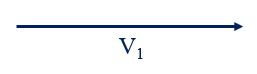
\includegraphics[scale=0.4]{figures/triunghi_viteza_ZAS.jpg}
	\caption{Triunghi viteză în zona aval-stator}
	\label{Triunghi viteză în zona aval-stator}
\end{figure}

\subsection{Alegerea razei de calcul a rețelelor}

Pentru proiectarea rețelelor de profile se calculează întâi raza medie a rețelelor la care se vor face în continuare calculele triunghiurilor de viteze. Se alege pentru aceasta o rază medie $R_m$ intre raza de periferie și raza de butuc astfel încât debitul dintre cele doua zone sa fie egale:

\begin{equation}
\frac{Q}{2} = V_a \pi (R_p^2 - R_m^2) 
\end{equation}

\begin{equation}
V_a \pi (R_p^2 - R_m^2) = 2 V_a \pi (R_p^2 - R_m^2) 
\end{equation}

\begin{equation}
R_p^2 - R_m^2 = 2 R_p^2 - 2 R_m^2
\end{equation}

\begin{equation}
R_m = \sqrt{\frac{R_p^2 + R_b^2}{2}} = \sqrt{\frac{0.110^2 + 0.094^2}{2}} = 0.102\si{m}
\end{equation}

În ZSR, avem viteza tangențiala $U$:

\begin{equation}
U = \omega R_m \text{ sau } \frac{\pi n}{30} R_m = \frac{\pi \cdot 1500}{30} 0.102 = 16.0 \si{m/s}
\end{equation}

Conform ecuației fundamentale a turbomașinilor (ecuația lui Euler) avem viteza absolută:

\begin{equation}
gH=UV_{u}, \text{ sau } gH=\frac{\pi n}{30} R_m V_{u}
\end{equation}

\begin{equation}
V_{u} = \frac{30gH}{\pi n R_m} = \frac{30 \cdot 9.81 \cdot 24 }{\pi \cdot 1500 \cdot 0.102} = 14.7 \si{m/s}
\end{equation}


Unghiul $\alpha_2$ dintre direcția tangențială și viteza absolută $V_u$ este:

\begin{equation}
tan(\alpha_{2 })=\frac{V_{u}}{V_{a}} = \frac{14.7}{6.8} \Rightarrow \alpha_{2}=65.1\si{\degree}
\end{equation}


Unghiul $\beta_2$ dintre direcția tangențială și viteza relativă $W_2$ este:

\begin{equation}
tan(\beta_{2})=\frac{U - V_u}{V_a} = \frac{16.0 - 14.7}{6.8} \Rightarrow \beta_{2} =11.0\si{\degree}
\end{equation}


\section{Triunghiurile de viteză}

Triunghiurile de viteză pentru ZSR se prezintă conform figurii 3.2.:

\begin{figure}[h!]
	\centering
	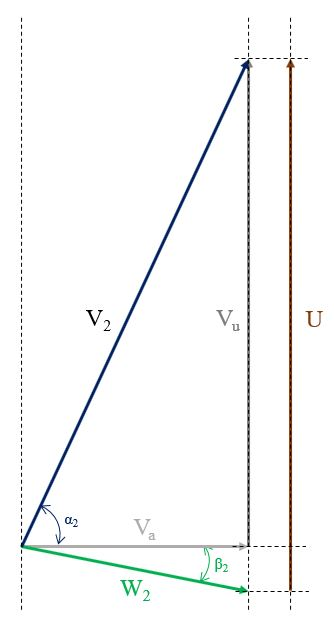
\includegraphics[scale=0.4]{figures/triunghi_viteza_ZSR.jpg}
	\caption{Triunghi viteză în zona stator-rotor}
	\label{Triunghi viteză în zona stator-rotor}
\end{figure}

\clearpage

Pentru ZAR avem aceleași viteză axială $V_a$ respectiv tangențială $U$. Putem calcula unghiul $\beta_3$ pentru a completa triunghiurile de viteză.

\begin{equation}
tan(\beta_{3})=\frac{U}{V_a} = \frac{16.0}{6.8} \Rightarrow \beta_{3} =66.9\si{\degree}
\end{equation}

\begin{figure}[h]
	\centering
	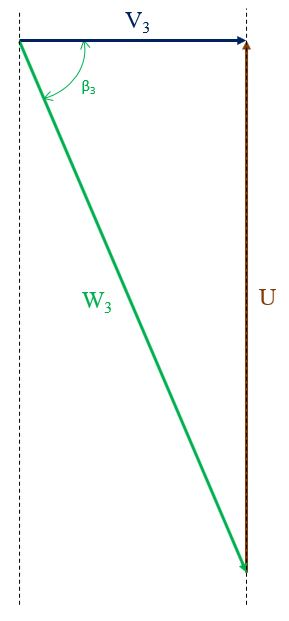
\includegraphics[scale=0.4]{figures/triunghi_viteza_ZAR.jpg}
	\caption{Triunghi viteză în zona aval rotor}
	\label{Triunghi viteză în zona aval rotor}
\end{figure}

\clearpage

\section{Alegerea pasului rețelei. Criteriul Zweifel}

Conform monografiei de Mecanica fluidelor și termodinamica turbomașinilor \cite{hall2013fluid}, pentru paletele de turbină există un raport pas-coarda optim care oferă un minim general de pierderi. Figura 3.4. ilustrează modul în care distribuția vitezelor variază în jurul suprafeței unei palete de turbine așezată în serie la trei valori ale pasului relativ.

\begin{figure}[h]
	\centering
	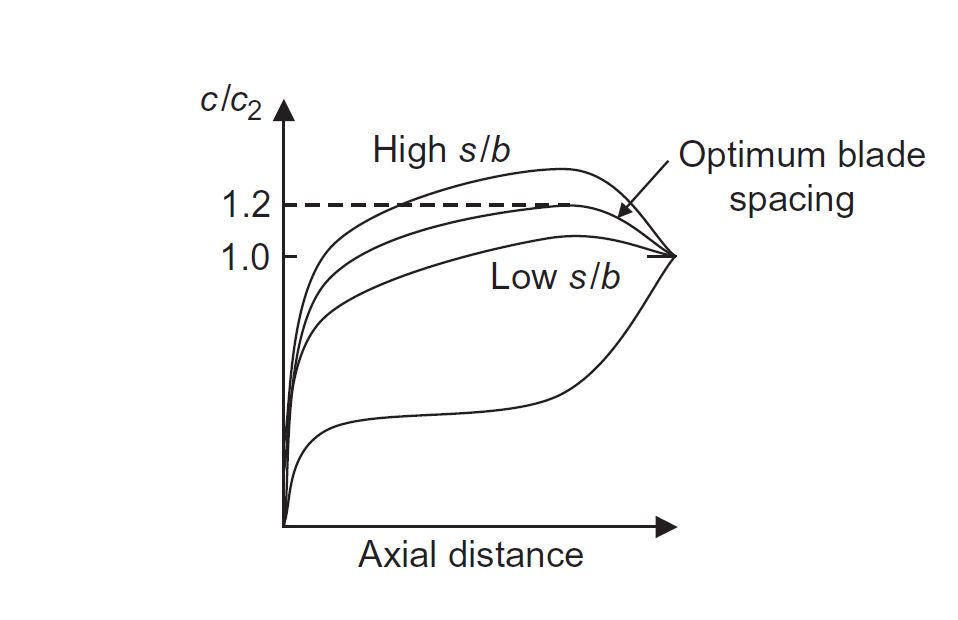
\includegraphics[scale=0.35]{figures/pasul_relativ_optim.jpg}
	\caption{Pasul relativ optim pentru o turbină \cite{hall2013fluid}}
	\label{Pasul relativ optim pentru o turbină}
\end{figure}

Pentru pas relativ mic, fluidul are un ghidaj maxim, dar pierderile prin frecare vor fi mari. Pe de altă parte, cu aceleași palete așezate la un pas mai mare, pierderile prin frecare sunt mici dar, din cauza ghidării defectuoase a fluidului, pierderile rezultate din separarea curentului sunt ridicate. Datorita acestor considerații, O. Zweifel \cite{zweifel1945frage} a formulat criteriul pentru raportul optim dintre pas și extensia axiala a paletei ce au unghiuri mari de deviere.

\begin{figure}[h]
	\centering
	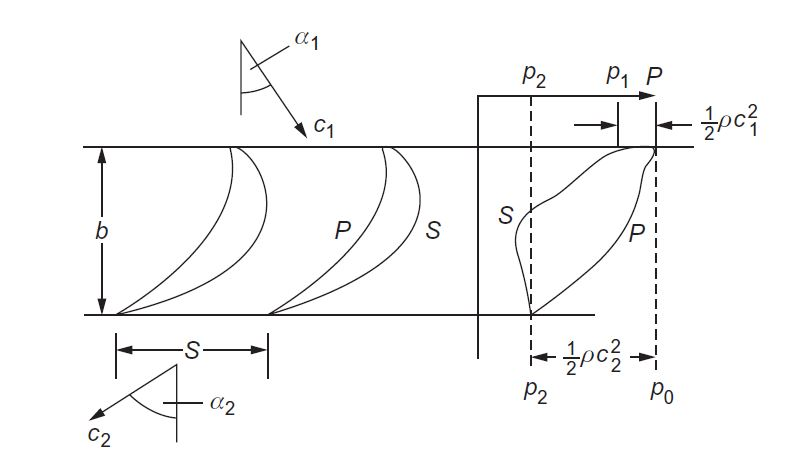
\includegraphics[scale=0.5]{figures/distributia_presiunii.jpg}
	\caption{Distribuție tipică a presiunii pe paleta de turbină \cite{hall2013fluid}}
	\label{Distribuție tipică a presiunii pe paleta de turbină}
\end{figure}

Figura 3.5. indică o distribuție tipică a presiunii într-o unei rețea de palete în turbină cu fluid incompresibil, curbele P și S corespunzătoare fetei de presiune (sau concavă), respectiv depresiune (convexă).

Zweifel a găsit empiric pentru turbine următoarea formula care depinde de unghiurile de intrare și de ieșire a fluidului în rețea:

\begin{equation}
Z_w = 2 \frac{s}{b} cos^2\alpha_2 (tan\alpha_1 + tan\alpha_2)
\end{equation}

La numere Mach mici, pentru pierderi minime a fost aproximata o valoare a $Z_w = 0.8$, astfel având stabilite unghiurile de intrare și de ieșire putem calcula pasul relativ în următorii pași:

\begin{equation}
0.8 = 2 \frac{s}{b} cos^2\alpha_2 (tan\alpha_1 + tan\alpha_2)
\end{equation}

\begin{equation}
\frac{s}{b} = \frac{0.4}{cos^2\alpha_2 (tan\alpha_1 + tan\alpha_2)}
\end{equation}

\begin{equation}
\frac{s}{b} = 0.4 \frac{1+tan^2\alpha_2}{tan\alpha_1 + tan\alpha_2}
\end{equation}

\begin{equation}
\frac{s}{b} = 0.4 \frac{1 + (V_u / V_a)^2 } {0 + (V_u / V_a)}
\end{equation}

\vspace{5mm} %5mm vertical space

Pentru stator $tan\alpha_1 = 0$ și ajungem la următorul rezultat:

\begin{equation}
(s/b)_{stator} = 0.4 \frac{1 + (14.7 / 6.8)^2 } {0 + (14.7 / 6.8)}\cong 1.05
\end{equation}

\vspace{5mm} %5mm vertical space

Pentru rotor avem urmatoarea ecuatie:

\begin{equation}
\frac{s}{b} = 0.4 \frac{1+tan^2\beta_3}{tan\beta_2 + tan\beta_3}
\end{equation}

\begin{equation}
\frac{s}{b} = 0.4 \frac{1 + (U / V_a)^2 } {(U - V_u) / V_a + (V_u / V_a)}
\end{equation}

\begin{equation}
(s/b)_{rotor} = 0.4 \frac{1 + (16 / 6.8)^2 } {(16 - 14.7) / 6.8 + (14.7 / 6.8)} \cong 1.03
\end{equation}

\clearpage


\section{Proiectare stator}

\subsection{Legea de încărcare}



\begin{figure}[h]
	\centering
	\includegraphics[scale=0.5]{figures/legea_de_incarcare.eps}
	\caption{Legea de încărcare}
	\label{Legea de încărcare}
\end{figure}


\begin{figure}[h]
	\centering
	\includegraphics[scale=0.5]{figures/stator_initial_blade.eps}
	\caption{Varianta inițială a geometriei paletei statorului}
	\label{Varianta inițială a geometriei paletei statorului}
\end{figure}

\begin{figure}[h]
	\centering
	\includegraphics[scale=0.5]{figures/stator_optimized_blade.eps}
	\caption{Varianta optimizată a geometriei paletei statorului}
	\label{Varianta optimizată a geometriei paletei statorului}
\end{figure}

\clearpage



\section{Proiectare rotor}

\begin{figure}[h]
	\centering
	\includegraphics[scale=0.5]{figures/stator_initial_blade.eps}
	\caption{Varianta inițială a geometriei paletei statorului}
	\label{Varianta inițială a geometriei paletei statorului}
\end{figure}

\begin{figure}[h]
	\centering
	\includegraphics[scale=0.5]{figures/stator_optimized_blade.eps}
	\caption{Varianta optimizată a geometriei paletei statorului}
	\label{Varianta optimizată a geometriei paletei statorului}
\end{figure}

\clearpage